\documentclass[a4paper]{article}
\usepackage[spanish]{babel}
\usepackage{hyperref}
\usepackage[utf8]{inputenc}
\usepackage{charter}
\usepackage{graphicx}
\graphicspath{ {img/} }

\usepackage{caratula}

%------------------------
\usepackage{color} % para snipets de codigo coloreados
\usepackage{fancybox}  % para el sbox de los snipets de codigo


% ********************************************************* %
% ~~~~~~~~         Formato de las páginas         ~~~~~~~~~ %
% ********************************************************* %


\usepackage{fancyhdr}
\pagestyle{fancy}

%\renewcommand{\chaptermark}[1]{\markboth{#1}{}}
\renewcommand{\sectionmark}[1]{\markright{\thesection\ - #1}}

\fancyhf{}

\fancyhead[LO]{Sección \rightmark} % \thesection\ 
\fancyfoot[LO]{\small{Lucas Iván Kruger, Franco Colombini, Gonzalo Monasterio}}
\fancyfoot[RO]{\thepage}
\renewcommand{\headrulewidth}{0.5pt}
\renewcommand{\footrulewidth}{0.5pt}
\setlength{\hoffset}{-0.8in}
\setlength{\textwidth}{16cm}
%\setlength{\hoffset}{-1.1cm}
%\setlength{\textwidth}{16cm}
\setlength{\headsep}{0.5cm}
\setlength{\textheight}{25cm}
\setlength{\voffset}{-0.7in}
\setlength{\headwidth}{\textwidth}
\setlength{\headheight}{13.1pt}
\setlength{\parskip}{2mm}
\renewcommand{\baselinestretch}{1.1}  % line spacing

%-----------------------

\title{Orga2 - tp2}
\author{ }
\date{May 2021}

\begin{document}
\thispagestyle{empty}
\materia{Organización del Computador II}
\submateria{Primer Cuatrimestre de 2021}
\titulo{Trabajo Práctico II}
\subtitulo{Implementación de filtros en SIMD}
\integrante{Lucas Iván Kruger}{799/19}{Lucaskruger10@gmail.com}
\integrante{Franco Colombini}{341/18}{francocolombini2013@gmail.com}
\integrante{Gonzalo Monasterio}{153/18}{gonzamonas@gmail.com}

\maketitle

\newpage

\thispagestyle{empty}
\vfill
\begin{abstract}
En el presente informe vamos a investigar el impacto del uso de simd en diferentes implementaciones de filtros de imágenes en ASM. Vamos a poner a prueba todas las implementaciones a través de el planteamiento de hipótesis y su debida experimentación. Todo el proceso, incluyendo la explicación de los algoritmos, hipótesis, experimentación, análisis y conclusiones son explicados en las secciones siguientes
\end{abstract}

\thispagestyle{empty}
\vspace{3cm}
\tableofcontents
\newpage


%\normalsize
\newpage

\section{Introducción}
En el siguiente informe mostramos como llevamos a cabo la implementación y experimentación de diferentes algoritmos de filtros de imágenes. El enfoque principal es ver si existe una mejora notable o no, respecto al uso de SIMD contra el uso de la implementación en C. 
Los tres filtros a implementar fueron Filtro Max, Filtro Gamma y Filtro Funny. Su explicación se encuentra en la sección implementación y en los comentarios de nuestro archivo de ASM.
Una vez implementados, experimentamos con los clocks obtenidos por cada implementación en diferentes tamaños de imágenes y los contrastamos haciendo uso de herramientas de análisis de datos, esto se explica en la parte de experimentación.
Las hipótesis son cuatro y son mostradas en la sección Hipótesis del trabajo, básicamente buscamos mostrar si hubo mejora entre nuestra implementación y la de c, cuanto aumentan los clocks en relación al tamaño de la imagen, cuanto afectan los accesos de memoria al rendimiento del programa, y si al tomar en cuenta el principio de vecindad espacial podemos generar algún aumento en rendimiento. En la sección resultados y análisis se puede ver esto con mas detalle.\\
En el apéndice se encuentran aquellas imágenes que sus resultados no consideramos tan significativos como para poner en el informe.



\section{Implementación}

\subsection{Filtro Max}
El filtro Max busca recorrer la imagen de a 4x4 píxeles, escribiendo en cada iteración la matriz 2x2 de su centro. Básicamente busca la máxima sumatoria de componentes RGB de un mismo píxel, entre los 16 de la submatriz 4x4, quedándose con la primer aparición en caso de que hayan varios iguales. Esto se hace dejando un marco de 1 píxel color blanco alrededor de toda la imagen.\\
En nuestra implementación lo primero que hacemos es colocar los bordes blancos. Ya que debemos operar de a al menos 2 píxeles a la vez y usando SIMD decidimos pintar el borde superior y el inferior de a 4 píxeles. Por otro lado, para pintar los costados tomamos los dos últimos píxeles de la fila de arriba y los dos primeros de la de abajo. Así podemos generar ambas franjas blancas y lo que sobra sera sobreescrito mas adelante. Para esto usamos un loop de filas, otro de columnas y el comando cmp para saber cuando pintar y cuando no. También creamos una mascara con el valor blanco repetido 4 veces para poder aplicarlo.\\
Para la parte de iteración en toda la imagen creamos dos loops, uno de filas y otro de columnas adentro de este. Al iterar columnas vamos avanzando de a 4 píxeles y en cada avance analizamos la submatriz 4x4 que queda en diagonal a este. Cabe destacar que tenemos dos registros MMX guardando el máximo global en sumatoria y el otro en píxeles que representan a esa sumatoria. En cada iteración hacemos dos pasos: búsqueda del máximo entre los 16 píxeles, y aplicación del máximo entre los cuatro píxeles del medio.\\

\begin{itemize}
\itemsep=0pt
    \item \textbf{Búsqueda del máximo entre los 16 píxeles:}\\
    \begin{itemize}
      \setlength\itemsep{0em}

     \item Primero actualizamos los máximos globales en cero (el de píxeles conserva el valor alpha en 255). \\
    \item Nos centramos en la primer fila de cuatro píxeles de la submatriz 4x4.\\
    \item Usamos mascaras para extraer los colores, separarlos y sumarlos de a 32 bits, para quedarnos con las cuatro sumas.\\
    \item Ahora buscamos el máximo de esta fila usando la instrucción pmaxud y shifteando, y lo ponemos en las cuatro posiciones de un xmm.\\
    \item Ahora que tenemos un xmmA con el max local en las cuatro posiciones es importante notar que mas adelante haremos uso de la función PHMINPOSUW, la cual busca el mínimo valor sin signo en WORDS en un xmm. Por lo que no pueden haber 0 en ninguna posición ya que sino lo tomaría como el máximo.\\
    \item Teniendo en cuenta esto le vamos a sumar a xmmA un 1 a todas las posiciones interpretadas en WORDS que no sean la posición en la que se guarda la sumatoria. Esto lo hacemos con la mascara dmask).\\
    \item Realizamos la comparación entre el máximo local (xmmA) y el registro que tiene las sumas de cada uno. IMPORTANTE: como sumamos 1s en el paso anterior(y por lo tanto comparan con 0), esto nos devolverá una mascara en WORDS con - 1 en aquellas posiciones donde la suma da el máximo. Guardamos en xmmA.\\
    \item Ahora teniendo nuestra mascara de a words seguimos la siguiente estrategia: 1- creamos 4 mascaras (imask's) en las que guardamos los valores que necesita la función PSHUFB para poder traer cada uno de los 4 valores de un xmm separado en DWORD. Estas mascaras están ordenadas en función de apuntar al primer DWORD, al segundo, etc. Y es importante ver que se ordenan de menor a mayor.\\
    \item Ahora aplicamos a las 4 imasks la mascara de xmmA y la función PHMINPOSUW, devolviéndonos así en un registro xmm que tiene en su parte baja los valores que apuntarían al valor que buscamos al aplicar PSHUFB.\\
    \item Realizamos un PACK de los cuatro xmm que tienen al mínimo y de esa manera obtenemos el valor que apunta al píxel en la parte baja. Ahora lo copiamos en las cuatro posiciones y utilizamos PSHUFB. Como resultado tenemos las componentes del píxel con la suma máxima local y primer aparición en las cuatro posiciones del registro dst.\\
    \end{itemize}
    \item \textbf{Aplicación del máximo entre los cuatro píxeles del medio:}
    \begin{itemize}
    \item Ya con ese valor copiado y teniendo aparte el máximo local, realizamos un pmax entre el máximo global en suma y el local, esto nos da una mascara de 0s o de -1s que después aplicamos a los cuatro valores del medio usándola. Si es la primer iteración aplica siempre y si es la segunda, tercera o cuarta solo aplicara en caso de que esa mascara quede en -1s. 
    \begin{figure}[htp]
    \centering
    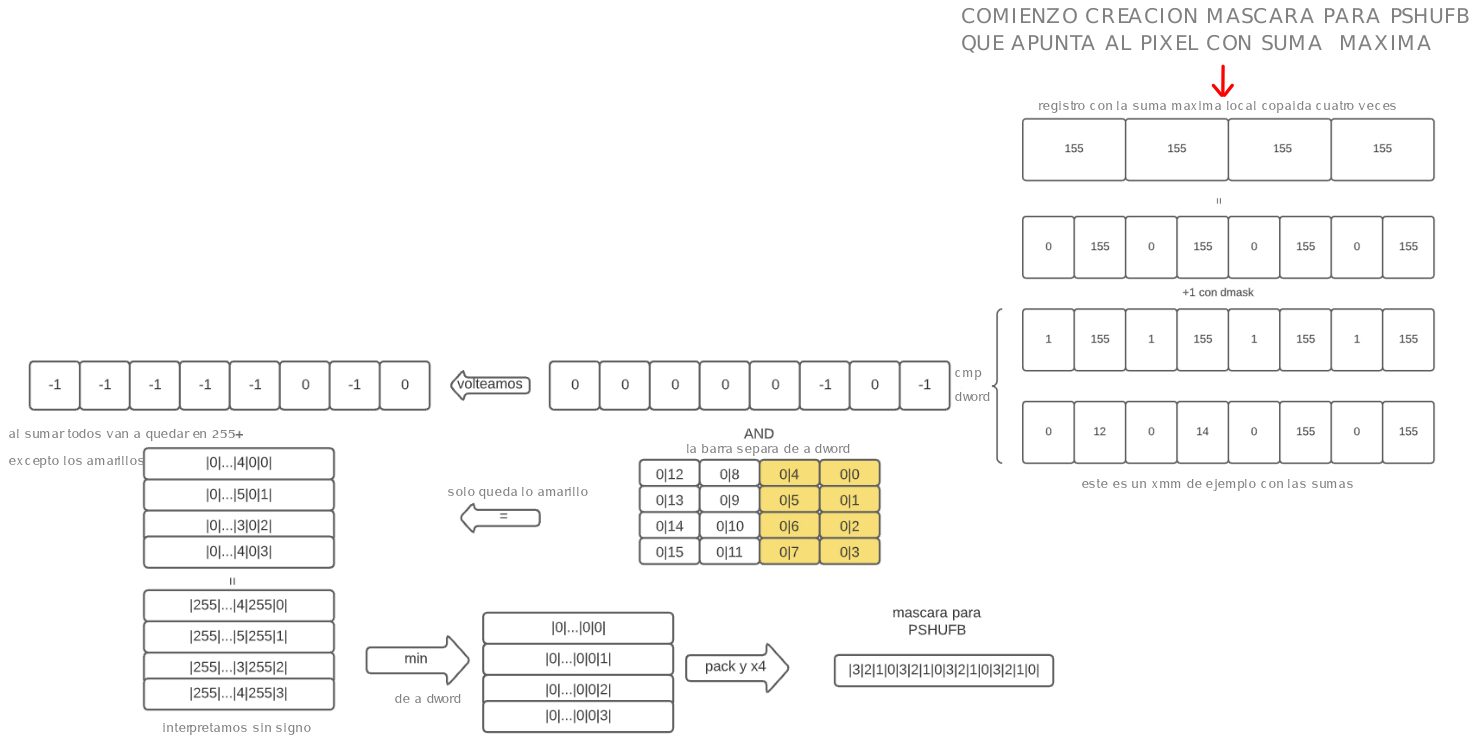
\includegraphics[scale=.26]{algofig.jpg}
    \caption{Ejemplo de como nuestra implementación de filtro max encuentra la mascara para pshufb al píxel con sumatoria mayor}
    \label{}
    \end{figure}
    \end{itemize}
    
\end{itemize}
  

\newpage


\subsection{Filtro Gamma}

Este filtro busca cambiar la gamma de la imagen, es decir la intensidad de los píxeles que la componen. Esto se hace aplicando la $Power Law Transform$, en particular usamos una simplificación de esta transformación (con parámetro $Gamma = 2$). La ecuación para cada componente de los píxeles de la imagen es $Output = 255*(Input\_matrix[i][j].color)^{1/Gamma}$.\\
Para la implementación del filtro Gamma utilizamos distintas mascaras para operar sobre cada color por separado. De esta forma nos aseguramos de no tener ningún problema de espacio para operar con los valores de cada color, en particular porque nos piden hacer varias operaciones de float, teniendo que convertir valores de 8 bits sin signo a valores float que ocupan 32 bits. Para operar extrajimos cada color con su mascara, y lo shifteamos un numero de bytes a derecha para que cada uno quede en la parte baja de su respectiva doubleword. Por ejemplo el color azul no fue shifteado ya que ya se encuentra en la parte baja de cada píxel, mientras que el verde fue shifteado 1 byte a derecha y el rojo 2 bytes a derecha.

Luego se realizaron las operaciones que indica el enunciado, y se guardaron los valores en un nuevo registro xmm, shifteando en cada caso para que cada color vuelva a estar en su lugar correspondiente. Para operar sobre los valores los transformamos a punto flotante y los volvimos a pasar a integer. Cabe mencionar que la cuenta expresada en el enunciado puede ser simplificada,  quedando finalmente en $\sqrt[2]{(255)src\_matrix[i][j].color}$, por lo que solo tuvimos que hacer una multiplicación y una raíz cuadrada.




\subsection{Filtro Funny}

Este filtro combina nuestra imagen de entrada con una nueva creada a partir de las coordenadas de cada píxel. Cada componente de píxel se calcula de forma independiente. En el caso del rojo tomamos la raíz cuadrada de la diferencia absoluta entre las dos coordenadas generando olas en ambos sentidos desde la diagonal de la imagen.
En el componente verde tomamos una división entre la suma y la resta de las coordenadas, agregando un factor de escala 10, creando rayos que se ven reflejados desde el 0:0 en adelante. Finalmente el componente azul genera una imagen curva debido a la multiplicación y luego raíz cuadrada de las coordenadas.

Para operar utilizamos distintas mascaras. En principio como operamos con cada color por separado utilizamos mascaras para separar cada color. Estos valores luego fueron convertidos a punto flotante y se les realizaron las operaciones detalladas en el enunciado. En los casos donde había que multiplicar o dividir por 10 y por 100 creamos unas mascaras especiales que guarden esos valores para luego poder multiplicarlos. En cada caso se transformaron los valores uint\_8 a punto flotante para poder operar y luego a integer de vuelta. Observamos que en el caso del azul tuvimos que trabajar con floats de doble precisión (doubles) ya que sino se perdía precisión respecto al programa de la cátedra. 



\section{Análisis Preliminar}


\section{Hipótesis de Trabajo}
Tenemos cuatro hipótesis:
\begin{itemize}

  
    \item \textbf{Comparación entre implementación ASM y C:} debido a que la implementación en ASM utiliza SIMD y recorre de a 4 píxeles esperamos que esta tenga una performance linealmente mejor que la versión de C la cual recorre de a 1.
    \item \textbf{Aumento de cantidad de píxeles:} Como nuestra implementación necesita operar sobre todos los píxeles de una imagen, esperamos que al tomar diferentes tamaños se obtenga un aumento proporcional en los clocks que usamos para aplicar el filtro.
    \item \textbf{Implementación con recorrido horizontal y vertical:} Todas las implementaciones de filtros en ASM recorren la imagen de forma horizontal, lo cual creemos que implica una mejora en el rendimiento ya que atiende al principio de vecindad espacial. Por lo anterior, pensamos que implementando algún filtro recorriendo de manera vertical obtendríamos una bajada en el rendimiento respecto al horizontal. Esto esperamos que se de sobre todo al aumentar el tamaño de una imagen ya que al dar saltos tan altos en memorias para iterar la cache tendría mayor cantidad de misses.
    \item \textbf{Costo de los accesos a memoria}
    Tenemos entendido que los accesos a memoria son bastante costosos en términos de rendimiento, por lo que imaginamos que si incrementamos el numero de accesos a memoria, por ejemplo guardando las mascaras de los filtros en cada iteracion de los loops en vez de al principio de cada programa, empeoraria notablemente el rendimiento de los filtros.
\end{itemize}


\section{Diseño experimental}
Para la experimentación se decidió realizar lo siguiente:

\begin{itemize}
    \item \textbf{Elección de set de imágenes:} Como nuestras hipótesis toman en cuenta el factor de cantidad de píxeles totales sobre los que operamos, decidimos tomar la imagen que se encuentra al final de esta sección de la pagina
     \href{https://www.pexels.com/es-es/foto/reflexion-de-la-montana-en-el-lago-braies-1525041/}{pexels.com}.\\
     Esta imagen tiene formato jpg y una resolución de 6000x4000, por lo que utilizamos la herramienta  \href{https://cloudconvert.com/bmp-converter}{https://cloudconvert.com/bmp-converter} que nos permitió convertirla a formato bmp y elegir el tamaño que buscábamos. Al final nos quedamos con un set de 9 tamaños diferentes: 24x16, 48x32, 96x64, 192x128 , 384x256, 768x512, 1536x1024, 6144 x 4096. Estos van multiplicando de a dos por lo que, de ser cierta nuestra hipótesis, implicaría un aumento exponencial en los clocks que necesita la implementación.

    \item \textbf{Modificación en Main para la obtención de muestras:} El main provisto por la materia nos permite ver cuantos clocks toma cada implementación. Lo que decidimos fue modificarla para que opere 50 veces y devuelva por consola una lista con las 50 mediciones de clocks. Esto es fundamental para después poder operar con ellas utilizando python.
    \item \textbf{Nueva implementación Gamma Vertical:} Para analizar nuestra tercer hipótesis decidimos tomar un filtro y ver si esta se cumple. Particularmente modificamos la implementación de Gamma y la llamamos Gamma-Vertical.La diferencia con la implementación de Gamma anterior es que la inicial recorre la imagen analizando conjuntos de píxeles de 4x4 y pasando al próximo conjunto de 4x4 que esta a la derecha, en cambio la versión vertical luego de procesar un conjunto de 4x4 píxeles pasa al que esta abajo. Básicamente cada vez que tiene que operar con los siguientes 4 píxeles tiene que dar un salto en memoria igual al ancho en bytes de la imagen multiplicado por 4.
    \item \textbf{Unidad de medición y donde se mide: } Optamos por el uso de clocks ya que permite comparar directamente el rendimiento. Todas las mediciones que son presentadas mas abajo fueron tomadas en una única computadora, buscando mantener las condiciones de ejecución (programas abiertos, etc.) lo mas óptimas posibles, buscando los mínimos outliers y obtener resultados con sentido entre si.
    \item \textbf{Herramientas de análisis y gráficos:} Para el análisis de los datos a obtener decidimos utilizar Python, en particular hicimos uso de las librerías numpy, pandas y matplotlib. Para una mejor visualización de los datos utilizamos gráficos como: boxplot (donde podamos ver tanto el promedio de los datos obtenidos, sus varianzas y outliers), barplot (donde podamos comparar relaciones entre las cantidades o proporciones obtenidas).
      %ACA VA LA IMAGEN
    \begin{figure}[htp]
    \centering
    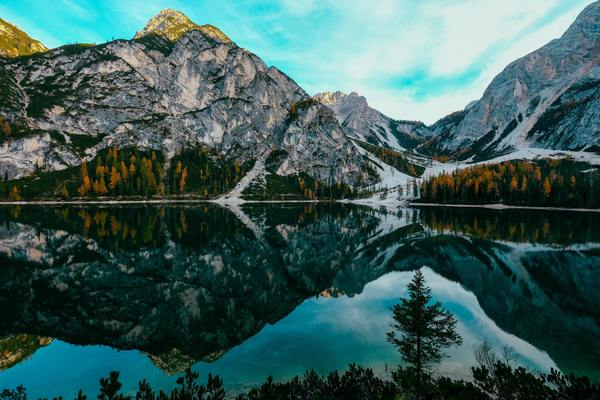
\includegraphics[scale=.5]{pexels-francesco-ungaro-1525041_50_1_20.jpg}
    \caption{Imagen tomada de pexels.com para experimentación.}
    \label{fig:galaxy}
\end{figure}
    
\end{itemize}


\section{Resultados y Análisis}
Los resultados y el análisis de datos serán presentado de la siguiente manera: comparación de implementaciones en ASM y C en diferentes tamaños de imagen y comparación entre Gamma y Gamma Vertical en diferentes tamaños de imágenes.
Primero que nada es importante aclarar que los resultados obtenidos presentaron una dispersión entre los datos que rondaba los miles. Esto era esperable debido a el numero de clocks que realiza un programa de esta índole y al hecho de que las mediciones son realizadas en una computadora de uso habitual atada al sistema operativo y los procesos en segundo plano.

\begin{itemize}
    \item \textbf{Comparación de implementación en ASM y C}:
    Para hacer este experimento armamos un Boxplot para cada filtro en el que le pasamos 100 mediciones (50 de ASM y 50 de C) por cada tamaño de imagen.
    En las figuras 3,4 y 5 podemos ver el aumento de clocks de las implementaciones para cada cantidad de píxeles. La linea azul conecta los promedios de las mediciones entre las implementaciones de ASM y la roja entre las de C.\\
    %[Aca podrian ir las tres imagenes,  voy a escribir la explicacion general, si quieren de a una agreguenlou 
    Como podemos ver hay claramente una cantidad menor de clocks en todas las implementaciones de ASM contra las de C. Esto respalda un poco mas nuestra hipótesis 1. Y puede de verse al uso de SIMD para procesar las imágenes.\\
    Además es importante notar que al principio la cantidad de clocks utilizadas es similar y luego se alejan. Esto se debe a que si la imagen es muy pequeña los clocks para operarla con registros de 64 bits o con registros SIMD son prácticamente despreciables, en el caso de la imagen de 24x16 ambas implementaciones usan una cantidad bajísima de ciclos. Al contrario cuando la imagen es muy grade si podemos sacar el máximo partido a SIMD, provocando una mejora apreciable debido a que pasamos a aplicar el filtro a miles de píxeles.\\
    Además podemos observar que el aumento que todas las implementaciones parece seguir el de una función con aumento exponencial, para comprobar esto aplicamos $log_2$ a todos los valores utilizados, obteniendo gráficos con aumentos similares al de una función lineal.
    Como observación final se puede ver como en las 3 figuras las cajas de los Boxplot son chatas, esto significa que los valores que no son outliers están cerca de la mediana.Y además, que a excepción de los clocks de la imagen mas grande a la que se le aplico Gamma, las figuras no presentan círculos los cuales representan outliers.
\\
    %Aca habria que poner los graficos, OSINO para que no quede tan lleno de graficos que dicen lo mismo, podemos poner un apoendice al final y ahi poner las imagenes. 
    Particularmente para cada caso, podemos ver que proporcionalmente la relación entre las implementaciones de ASM y C son las siguientes: en Max ASM fue un 78.1\% mas rápido; en Gamma ASM fue un 71.5\% mas rápido; y en Funny fue un 89.9\% mas rápido. Esto lo medimos tomando el promedio de los clocks obtenidos para cada tamaño de imagen.
    %aca iria grafico de barras mostrando en porcentaje cuanto porciento es la asm de C, o simplemente calcular los tres vaores y escribirlos.
    
\begin{figure}[htp]
    \centering
    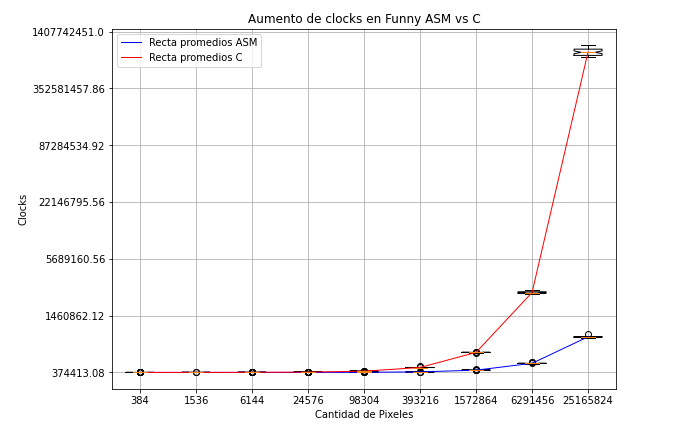
\includegraphics[scale=.5]{BoxplotFunnyAsmvsC.png}
    \caption{Aumento de clocks en Funny ASM vs C}
    \label{fig:galaxy}
\end{figure}

\begin{figure}[htp]
    \centering
    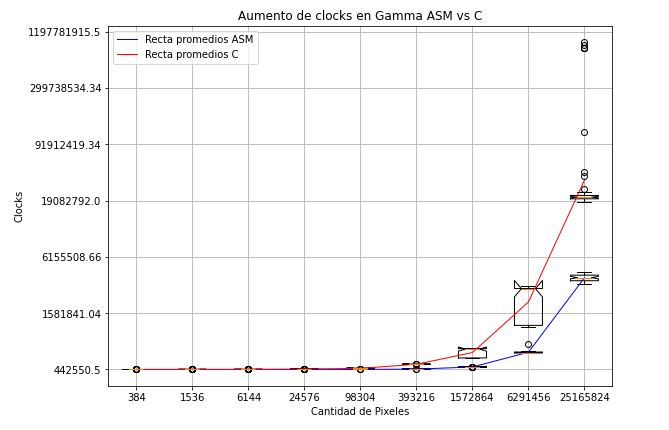
\includegraphics[scale=.5]{BoxPlotGammaCvsAsm.png}
    \caption{Aumento de clocks en Gamma ASM vs C}
    \label{fig:galaxy}
\end{figure}

\begin{figure}[htp]
    \centering
    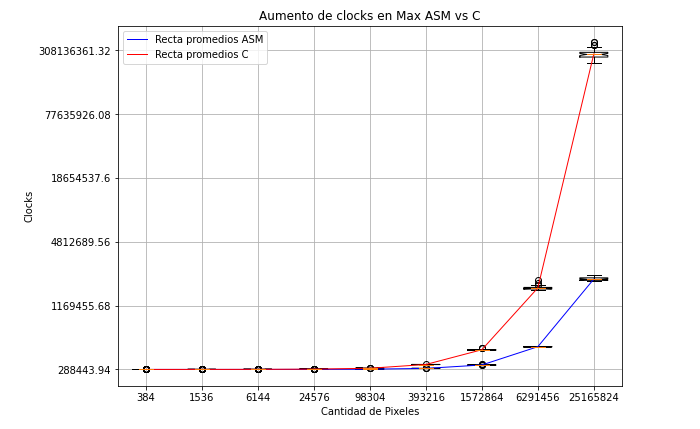
\includegraphics[scale=.5]{BoxplotMaxCvsASM.png}
    \caption{Aumento de clocks en Max ASM vs C}
    \label{fig:galaxy}
\end{figure}

\newpage
    \item \textbf{Gamma Vertical en diferentes tamaños de imágenes:} 
    El siguiente gráfico es muy similar a los utilizados en la sección anterior, solo que comparamos la implementación de ASM que recorre de forma vertical y la que recorre de manera horizontal.\\
   
    
    Como podemos ver las diferencias entre implementaciones son bastante pequeñas. Esto puede deberse al tamaño de la cache o a las predicciones que realiza el sistema a la hora de tomar valores en memoria que podrían llevar a una mejora en el rendimiento. Esto muestra ciertos puntos no tomados en cuenta en nuestra hipótesis. 
    Dado que los valores usados son muy grandes y las diferencias difíciles de ver a simple viste decidimos armar el siguiente gráfico:
    

     \begin{figure}[htp]
    \centering
    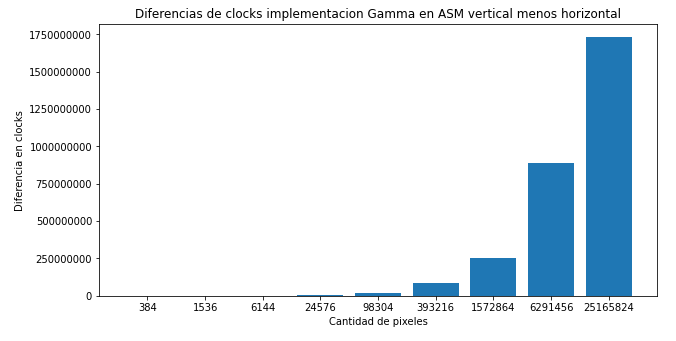
\includegraphics[scale=.66]{BarPlot.png}
    \caption{Diferencia de clocks implementación Gamma en ASM vertical menos implementación horizontal}
    \label{}
    \end{figure}
    %grafico de barras donde hacemos horizontal - vertical
    En este gráfico tomamos las medias obtenidas en cada muestra y las restamos para obtener su diferencia. Específicamente hicimos  ClocksVertical - ClocksHorizontal y no tomamos el valor absoluto ya que queríamos saber cual implementación fue la que mas tardo. Todos los valores arrojados fueron positivos por lo que muestran que los clocks usados para la implementación vertical fueron mayores. Mas aun, estos clocks fueron aumentando con el aumento de el tamaño de la imagen, lo cual si tiene relación con nuestra hipótesis 3. Esto puede deberse justamente a que a pesar de las optimizaciones que el sistema pueda hacer para el uso de la cache, estas van perdiendo efectividad al tener que operar con cantidades de memorias mas grandes que pueden llegar a superar lo que la cache almacena y rompiendo el principio de vecindad espacial.
    
    
    \item \textbf{Costo de los accesos a memoria}
    
    Para este experimento quisimos ver como impactan los accesos a memoria al rendimiento de los filtros. Nuestra hipótesis es que los accesos a memoria son muy costosos. Para verlo tomamos la función Funny, que utiliza una gran cantidad de máscaras que son guardadas en registros XMM antes de comenzar los ciclos del programa y simplemente movimos estos accesos a memoria dentro del ciclo principal del programa, para que se ejecuten en cada iteración del ciclo. Estos experimentos fueron corridos sobre la imagen en tamaño 1536x1024. En total pasamos 6 mascaras adentro del ciclo: bluemask, greenmask, redmask, amask, maskj, mask100. Las mascaras mask100 y mask10 no fueron pasadas ya que se les ejecuta una conversion de integer a float que al ponerla dentro del ciclo afectaría la performance y solo nos interesan los accesos a memoria.
    Los resultados fueron los siguientes:
    
    Promedio de Funny sin accesos extra de memoria : 14217550 ciclos.
    
    
    Promedio de Funny con accesos de memoria dentro del ciclo: 14237026 ciclos.
    
     Como se puede ver no hubo una gran diferencia en el rendimiento del filtro respecto al numero de accesos a memoria. Esto puede significar que los accesos a memoria no son tan costosos como nosotros pensábamos, o también puede ser que la cache guarde estos accesos a memoria y entonces no tenga que acceder todo el tiempo sino que ya tenga esos valores guardados.
    
        
    


\end{itemize}
\section{Experiencias al programar:} La implementación de los diferentes algoritmos implicaron superar diferentes dificultades:
\begin{itemize}
    \item \textbf{Filtro Max:} Su implementación fue la mas difícil por varias razones: 
    \begin{itemize}
        \item -Pintar borde de blanco: Primero optamos por pintar la imagen entera de blanco, lo cual era contraproducente para la performance del sistema. Al final decidimos cambiar el algoritmo por uno mejor que solo pinta cuando es necesario.
        \item -Búsqueda del máximo: El mayor obstáculo que presento este ejercicio fue como relacionar la suma máxima de los componentes de un píxel con su píxel correspondiente cuando hay mas de un píxel con la misma suma y ambos son el máximo. Al principio nos estancamos y pensamos incluso en una implementación con un loop, lo cual era erróneo y gracias a la ayuda de nuestro corrector pudimos solucionar.
    \end{itemize}
    \item \textbf{Filtro Gamma:} Su implementación fue la mas sencilla ya que solo era la aplicación de diferentes operaciones a cada valor de píxel. Cabe destacar que por su sencillez fue el algoritmo optado para experimentar cambiando su iteración de horizontal a vertical. %yo no labure aca, si falta algo agregar
    \item \textbf{Filtro Funny:} Su implementación en un principio pareció fácil pero trajo ciertos problemas: 
    \begin{itemize}
        \item Conversiones a punto flotante y a enteros: Aprendimos mucho de esta parte y de como utilizar el truncamiento. En un principio hacíamos eso al final, lo cual nos llevaba a imágenes diferentes a las deseadas.
        \item Uso de doubles en azul: debido a una diferencia a la hora de aplicar el truncamiento, tuvimos que resolver los cálculos de este color usando doubles. En un principio usábamos punto flotante normal pero eso nos llevaba a errores en unos pocos tests.
    \end{itemize}
    
\end{itemize}
\section{Conclusiones}

Pudimos observar que al menos dos de nuestras tres hipótesis parecían ser mas acertadas. La tercera y la cuarta quizás necesitaron tener en cuenta mas factores que pudimos ver al experimentar. 
Concluimos que las implementaciones en C presentan menor rendimiento contra las realizadas en ASM haciendo uso de SIMD. 
También concluimos que el aumento en ciclos de reloj que va a tener nuestra implementación es directamente proporcional al aumento de píxeles de la imagen a procesar.

Por ultimo vimos que si hay una mejora al utilizar una implementación que se beneficia del principio de vecindad espacial, y que este beneficio aumenta conforme aumentamos los píxeles a procesar. Pero también vimos que este aumento no es tan grande como esperábamos, debido quizás a las optimizaciones realizadas por el sistema donde fue implementado y mas particularmente a los sistemas de predicción que este usa en la cache.

Algunas propuestas para futuros experimentos serian: las mismas mediciones en algún entorno mas controlado, experimentar con diferentes colores usados en las imágenes elegidos de forma arbitraria, la comparación entre la implementación c y otra en ASM pero con registros normales, y la realización de experimentos con los demás filtros recorridos de manera vertical.

El uso de simd nos lleva a una gran mejora en el rendimiento en casos donde hay que procesar muchos datos a la vez, y el aprovechamiento de ciertos criterios como el de vecindad espacial también.

\section{Apendice}
Aquí se encontraran aquellas imágenes que creimos que eran importantes pero no lo suficiente para estar en el medio del informe.
\begin{figure}[htp]
    \centering
    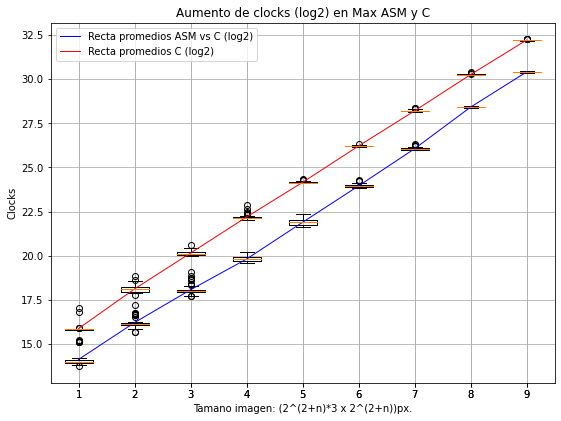
\includegraphics[scale=.5]{log21.jpg}
    \caption{Aumento de clocks en Max usando log2}
    \label{fig:galaxy}
\end{figure}

\begin{figure}[htp]
    \centering
    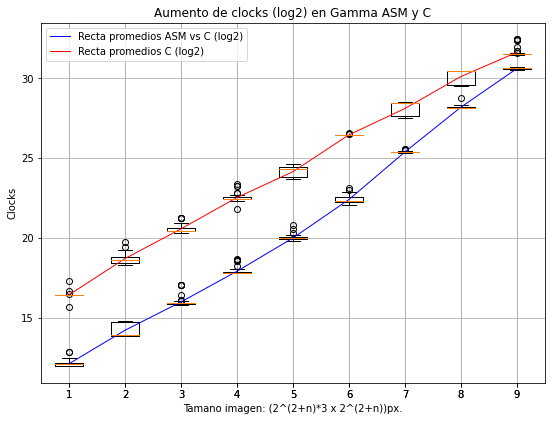
\includegraphics[scale=.5]{log22.jpg}
    \caption{Aumento de clocks en Gamma usando log2} 
    \label{fig:galaxy}
\end{figure}

\begin{figure}[htp]
    \centering
    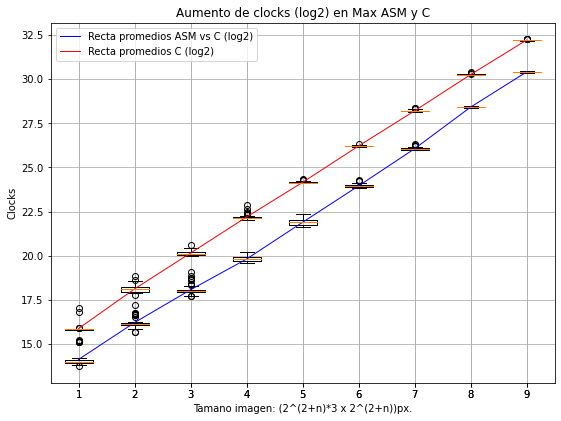
\includegraphics[scale=.5]{log21.jpg}
    \caption{Aumento de clocks en Funny usando log2}
    \label{fig:galaxy}
\end{figure}
\begin{figure}[htp]
    \centering
    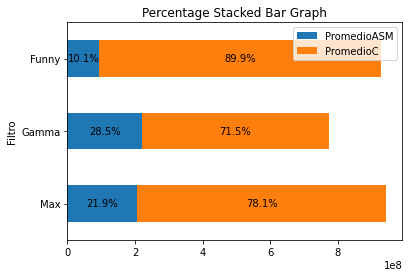
\includegraphics[scale=.5]{barras.jpg}
    \caption{Gráfico de barras comparando ASM y C}
    \label{fig:galaxy}
\end{figure}


\end{document}
